\documentclass{article} % For LaTeX2e
\usepackage{nips15submit_e,times} % Example is in "nips15.tex"
\usepackage{hyperref}
\usepackage{url}
\usepackage{algpseudocode,algorithm,algorithmicx}  
\usepackage[square,sort,comma,numbers]{natbib}

\usepackage{graphicx}
\usepackage{caption}
\usepackage{subcaption}
%\usepackage[outdir=./figures/]{epstopdf}
\usepackage{amsmath}
\usepackage{amsfonts}
%\documentstyle[nips14submit_09,times,art10]{article} % For LaTeX 2.09

\title{Gaussian Process Bandits}

\author{
Emile Mathieu \\ %\thanks{ Use footnote for providing further information
%about author (webpage, alternative address) \\
Department of Computer Science\\
Ecole des Ponts ParisTech\\
\texttt{emile.mathieu@eleves.enpc.fr} \\
}

\newcommand{\fix}{\marginpar{FIX}}
\newcommand{\new}{\marginpar{NEW}}

\nipsfinalcopy % Uncomment for camera-ready version

\begin{document}

\maketitle

\begin{abstract}
A lot of applications require to optimize black-box, noisy function that is expensive to evaluate.
This task can be formulated as a multi-armed bandit problem, where the reward function is sampled from a Gaussian Process (GP) or has low RKHS norm.
%Learning in a bandit setting when the reward is a function $f$ of the arm’s contexts such that $f \sim$ GP.
This setting was first studied by \citet{DBLP:conf/icml/SrinivasKKS10}, where the authors proposed GP-UCB, a UCB-like algorithm.
We propose a Thompson sampling algorithm adapted for this setting.
\end{abstract}

\section{Introduction}

\subsection{Problem Statement}
The problem we consider is the sequential optimization of an unknown reward function $f : D \rightarrow \mathbb{R}$.
At each round $t$, we choose a point $\mathbf{x}_t \in D$ and get to observe the function value perturbed by noise: $y_t = f(\mathbf{x}_t) + \epsilon_t$.
Our goal is to perform as well as $\mathbf{x}^\star = \arg\max_{\mathbf{x} \in D}  f(\mathbf{x})$, which is maximizing the sum of rewards $\sum_t^T f(\mathbf{x}_t)$.

In bandit settings, the natural performance metric is the cumulative regret, which is the loss in reward due to not knowing $f$'s maximum.
Formally, the cumulative regret $R_T$ after $T$ rounds is the sum of instantaneous regret: $R_T = \sum_t^T r_t$, with $r_t = f(\mathbf{x}^\star) - f(\mathbf{x}_t)$.

\subsection{Related work}




\section{Gaussian Processes}
\subsection{Overview}
For a nice introduction of Gaussian Process applied to Bayesian optimization see \citet{Brochu:2009}. GP can be seen as an extension of the multivariate Gaussian distribution (as this distribution is a generalization of the univariate Gaussian) to an infinite-dimension distribution for which any finite combination of dimensions will be a Gaussian distribution. In this manner, a GP is a distribution over functions, completely specified by a mean function $\mu$ and a covariance function $k$: $\forall \mathbf{x} \in \mathcal{D}$
$$ f(\mathbf{x}) \sim \mathcal{GP} \left(\mu(\mathbf{x}), k(\mathbf{x},\mathbf{x}') \right) $$

%$\forall \ [\mathbf{x}_1, \dots, \mathbf{x}_T] \in \mathcal{D}^T$

Common choices of covariance functions are:
\begin{itemize}
\item Finite dimensional linear: $k(\mathbf{x}, \mathbf{x'}) = \mathbf{x}^T \mathbf{x'}$

\item Squared Exponential kernel: $k(\mathbf{x}, \mathbf{x'}) =  \exp \{ -(2l^2)^{-1} {\left\| \mathbf{x} - \mathbf{x'} \right\|}^2 \}$

\item Matern kernel: $k(\mathbf{x}, \mathbf{x'}) = (2^{1- \nu} / \Gamma(\nu)) r^\nu B_\nu(r)$, $r= (\sqrt{2 \nu} / l) \left\| \mathbf{x} - \mathbf{x'}\right\|$

\end{itemize}

\subsection{Gaussian Processes reward functions}
Gaussian Processes (\citet{Rasmussen:2005:GPM:1162254}) allow smoothness assumptions about the reward function $f$ to be encoded through the choice of kernel in a flexible non parametric way.

Here, the reward function $f$ can be assumed to come from a GP, and perturbed with gaussian noise:  $y=f(\mathbf{x}) + \epsilon$, with $\epsilon \sim \mathcal{N}(0, \sigma^2)$ and $ f \sim$ GP$(0_d, k(\cdot,\cdot))$. Hence $y = (f+\epsilon) \sim$ GP$(0_d, k(\cdot,\cdot) + \sigma^2)$.
The reward can also be assumed to have low RKHS norm.

Either way, algorithms (GP-UCB and GP-TS) uses a GP$(0_d, k(\cdot,\cdot))$ as a prior distribution over $f$.

%GP prior $GP(0, k(\mathbf{x}, \mathbf{x'}))$

\section{Bandit's Algorithms}

\subsection{GP-UCB}
\citet{DBLP:conf/icml/SrinivasKKS10} introduces an upper-confidence based algorithm named Gaussian Process-Upper Confidence Bound (GP-UCB) which is detailed in Algorithm \ref{alg:gp-ucb}.
At each time step $t$, it chooses
$$\mathbf{x}_t = \arg\max_{\mathbf{x} \in \mathcal{D}} \mu_{t-1}(\mathbf{x}) + \sqrt{\beta_t} \sigma_{t-1}(\mathbf{x})$$
This choice implicitly negotiates the exploration-exploitation trade-off.
It can be interpreted as greedily selecting points $\mathbf{x}$ such that $f(\mathbf{x})$ should be a reasonable upper bound on $f(\mathbf{x}^\star)$.

This selection rule is motivated by the UCB algorithm for the classical multi-armed bandit problem (\citet{Auer:2003:UCB:944919.944941, Kocsis:2006:BBM:2091602.2091633}).

\begin{algorithm}  
  \caption{GP-UCB
    \label{alg:gp-ucb}}  
  \begin{algorithmic}[1]  
    \Require{$k$}  
    \State  $\mu \gets 0_d$
      \For{$t \gets 1 \textrm{ to } T$}  
          \State  $\beta_t \gets 2 \log (\left| D \right| t^2 \pi^2 / 6 \delta)$
    \State Choose $a_t \gets arg \max_i \mu_{t-1} + \sqrt{\beta_t} \sigma_{t-1}$
    \State Observe $y_t = f(\mathbf{x}_t) + \epsilon_t$
    \State $\mu_t = k_{t-1}(\mathbf{x})^T {(K_{t-1} + \sigma^2 I_d)}^{-1} y_t$
    \State $k_t = k(\mathbf{x}, \mathbf{x}') - k_{t-1}(\mathbf{x})^T {(K_{t-1} + \sigma^2 I_d)}^{-1} k_{t-1}(\mathbf{x'}) $
    \State $\sigma_{t}^2 = k_t(\mathbf{x},\mathbf{x})$
      \EndFor  
  \end{algorithmic}  
\end{algorithm}

\subsection{GP-TS}

Thompson Sampling (TS) is one of the earliest heuristics for multi-armed bandit problems.
The first version of this Bayesian heuristic dates to \citet{thompson1933}.
It is a member of the family of \textit{randomized probability matching} algorithms.

%Thompson Sampling is a randomized algorithm based on Bayesian ideas.
The main idea is to assume a prior on parameters $\theta$ of the reward function and to update these parameters by computing the posterior distribution $P(\theta | \mathcal{D}_{1:t})$ after observing a reward. At each time step $t$, the algorithm plays an arm according to its posterior probability of being the best arm.

A generalization of Thompson Sampling algorithm for the stochastic contextual multi-armed bandit problem with linear pay-off functions is given by \citet{DBLP:conf/icml/AgrawalG13}.

We propose a generalization of Thompson Sampling algorithm for the stochastic multi-armed bandit problem with reward functions sampled from GP. In this setting, the elements of Thompson sampling are as follows:
\begin{itemize}
\item The set $\Theta$ of parameters $\theta$ of the distribution of $f$ is the set of tuples $\left\{ \mu( \cdot ), k(\cdot,\cdot) \right\}$, with $\mu : \mathcal{D} \rightarrow \mathbb{R}$ and $k : \mathcal{D} \times \mathcal{D} \rightarrow \mathbb{R}$.

\item The prior distribution $P(\theta)$ on those parameters is a gaussian process: $f \sim$ GP$(\mu_0( \cdot ), k_0(\cdot,\cdot))$.
Without loss of generality\footnote{According to \citet{Rasmussen:2005:GPM:1162254}}, we assume $\mu_0 = 0_d$.

\item We observe triplets $\mathcal{D} = {\left\{\mathbf{x}; y \right\}}_t$.

\item At each step $t$, the reward $y_t$ comes from $y_t=f(\mathbf{x}_t) + \epsilon$, with $\epsilon \sim \mathcal{N}(0, \sigma^2)$. Thus 
$$ (f+\epsilon) \sim \text{GP}(\mu( \cdot ), k(\cdot,\cdot) + \sigma^2)$$
Consequently, the likelihood function is 
$$P(y | \theta, \mathbf{x}) = \frac{1}{\sqrt{2 \pi (\sigma_t^2 + \sigma^2)}}\exp \left\{ -  \frac{ {(\mathbf{x} - \mu_t)}^2 }{2 (\sigma_t^2 + \sigma^2)} \right\}$$

\item The posterior distribution $P(\theta | \mathcal{D}_{1:t}) \propto P(\mathcal{D}_{1:t} | \theta) P(\theta)$ yields the following update on (functions) parameters $\left\{ \mu( \cdot ), k(\cdot,\cdot) \right\}$: 
	\begin{itemize}
	\item $\mu_t = k_{t-1}(\mathbf{x})^T {(K_{t-1} + \sigma^2 I_d)}^{-1} y_t$
	\item $k_t = k(\mathbf{x}, \mathbf{x}') - k_{t-1}(\mathbf{x})^T {(K_{t-1} + \sigma^2 I_d)}^{-1} k_{t-1}(\mathbf{x'}) $.
	\end{itemize}
\end{itemize}

The proposed GP-TS algorithm is summed up in pseudo-code in Algorithm \ref{alg:gp-ts}.

\begin{algorithm}  
  \caption{GP-TS
    \label{alg:gp-ts}}  
  \begin{algorithmic}[1]  
    \Require{$k$}  
    \State  $\mu \gets 0_d$
      \For{$t \gets 1 \textrm{ to } T$}  
          \State  Sample $f_t \sim \mathbf{GP}(\mu_t, K_t) $
    \State Choose $a_t \gets arg \max_a f_t(\mathbf{x}_{a,t})$
    \State Observe $y_t = f(\mathbf{x}_t) + \epsilon_t$
    \State $\mu_t = k_{t-1}(\mathbf{x})^T {(K_{t-1} + \sigma^2 I_d)}^{-1} y_t$
    \State $k_t = k(\mathbf{x}, \mathbf{x}') - k_{t-1}(\mathbf{x})^T {(K_{t-1} + \sigma^2 I_d)}^{-1} k_{t-1}(\mathbf{x'}) $
    \State $\sigma_{t}^2 = k_t(\mathbf{x},\mathbf{x})$
      \EndFor  
  \end{algorithmic}  
\end{algorithm}

\subsection{Kernel learning\label{kernel_learning}}


Once a parametrized kernel has been selected for the GP prior over $f$, one need to choose its parameters. For a squared exponential kernel
$k(\mathbf{x}, \mathbf{x'}) = \exp \{ -(2l^2)^{-1} {\left\| \mathbf{x} - \mathbf{x'} \right\|}^2 \}$
, the lengthscale $l$ is a parameter to be tuned. 

A classical way to do so is to compute the log likelihood and to find parameters which maximizes it.
These parameters are then called maximum likelihood estimators (MLE).
For the squared exponential kernel, because $y_t =$ the log likelihood is the following:
$$ \mathcal{N}(\mathbf{y} | 0, \mathbf{K}) = {(2 \pi)}^{-n/2} {|\mathbf{K}+ \sigma^2I |}^{-1/2} \exp \{ -\mathbf{y}^T {(\mathbf{K}+ \sigma^2 I)}^{-1} \mathbf{y} \} $$

with $\mathbf{y}=[y_1, \dots, y_T]^T $ and $\mathbf{K}$ the positive definite kernel matrix $[k(\mathbf{x}, \mathbf{x'})]_{\mathbf{x}, \mathbf{x'} \in A_T}$.
This MLE problem can then be formulated as the following otpimization problem:
$$ l^\star \in \arg\min E(l) $$
$$ \text{with} \quad E(l) = \frac{1}{2} \log |\mathbf{K}+ \sigma^2 I | + \frac{\mathbf{y}^T {(\mathbf{K}+ \sigma^2 I)}^{-1} \mathbf{y}}{2} \propto -\log \mathcal{N}(\mathbf{y} | 0, \mathbf{K}) $$

\section{Experiments}
\subsection{Compared methods}
We compare performances between GP-UCB, GP-TS and two naives methods which choose points of maximum mean or variance only, both on synthetic and real sensor network data.

\textcolor{red}{The code of experiments is available online at}

% Maximum Expected Improvement ( Mockus et al. 1978) 
% Most Probable Improvement (Mockus 1989)

\subsection{Synthetic data}
For synthetic data, we use the same procedure and parameters as in \cite{DBLP:conf/icml/SrinivasKKS10}. Hence, we sample random functions from a GP with a squared exponential kernel with lengthscale parameter $l=0.2$. The sampling noise variance $\sigma^2$ was set to $0.025$. Our decision set $D = [0, 1]$ is uniformly discretized into $1000$ points.

First, we learn the lengthscale of the squared exponential kernel with the method described in the Kernel Learning subsection. We discretize the lengthscale space, compute $E(l)$ for each lengthscale $l$ and return the lengthscale $l$ which minimizes $E(l))$. These values $E(l)$ are plotted in blue in Figure \ref{kernel_learning}, and the best lengthscale $l^\star$ is represented by a vertical red dashed line.


Then, we run each algorithm for $T = 100$ iterations with $\delta = 0.1$ and $l=l^\star$, averaging over 150 trials (samples from the kernel). We follow the choice of $\beta_t$ as recommended by Theorem 1 in \cite{DBLP:conf/icml/SrinivasKKS10}, which is $\beta_t = 2 \log (|D| t^2 \pi^2/6 \delta)$. Obtained results are shown in Figure \ref{synthetic_data}.
%mean average regrets are computed by averaging regrets on those samples.

\begin{figure}[h!]
  \begin{subfigure}[b]{0.5\linewidth}
    \centering 
    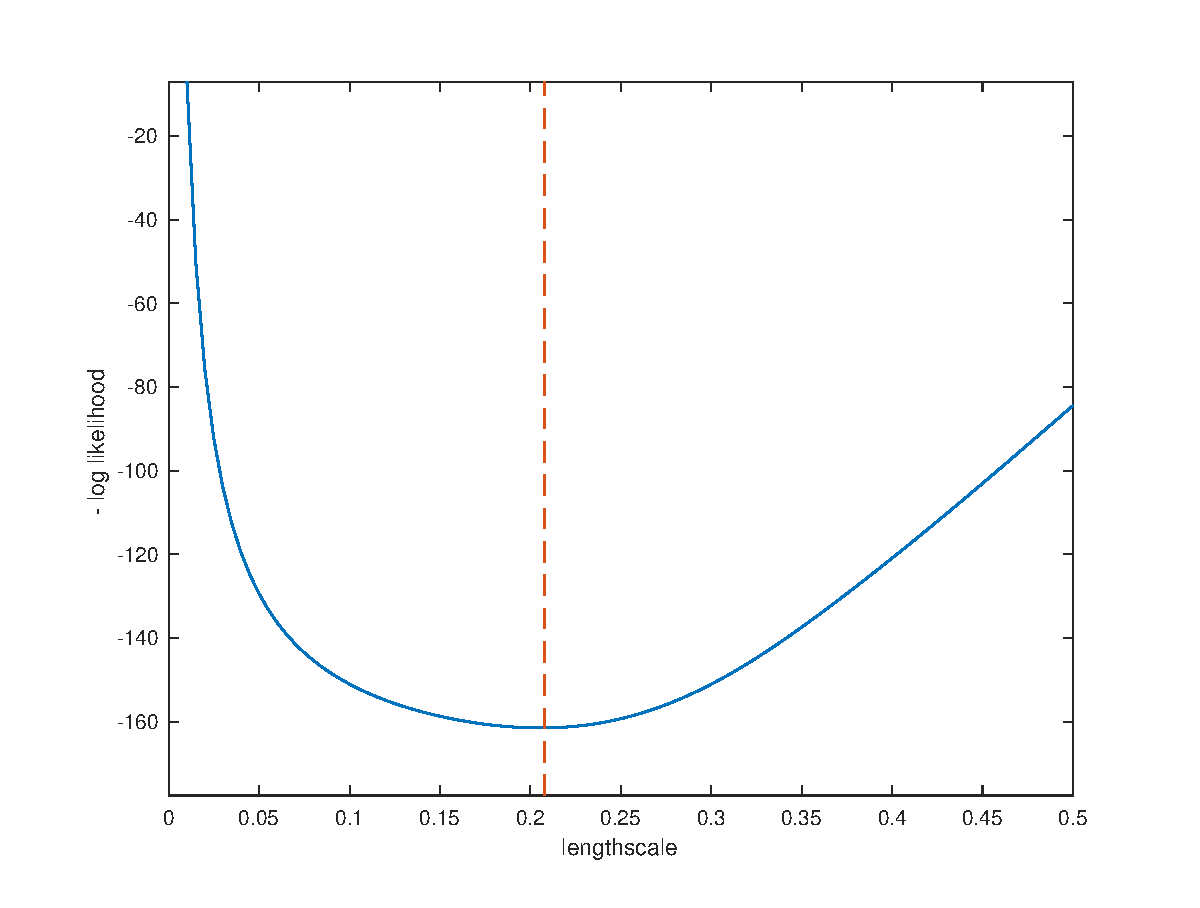
\includegraphics[width=1\linewidth]{figures/synthetic_lengthscale_learning.eps} 
    \caption{Kernel's lengthscale learning} 
    \label{kernel_learning} 
    \vspace{4ex}
  \end{subfigure}
  \begin{subfigure}[b]{0.5\linewidth}
    \centering
    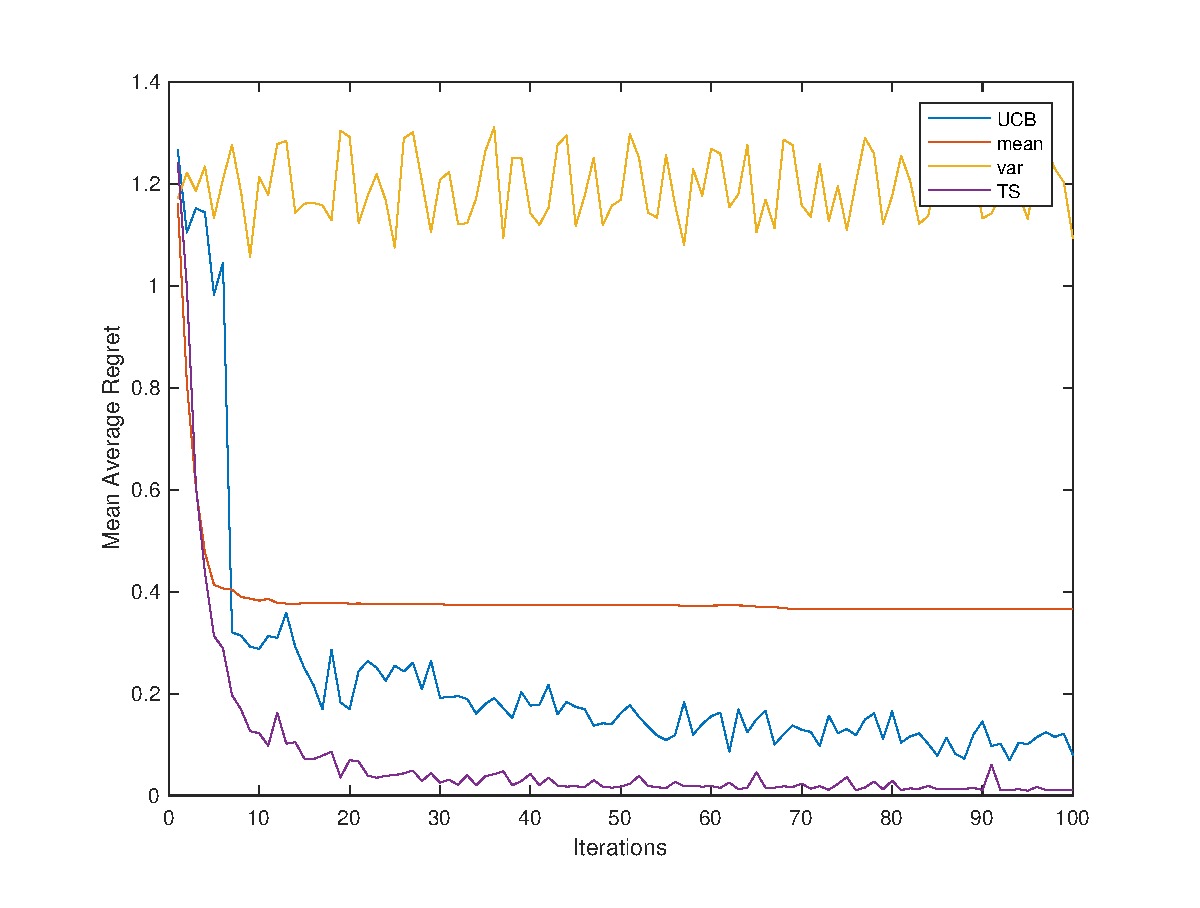
\includegraphics[width=1\linewidth]{figures/synthetic_MC_150_kernel_sqe.eps} 
    \caption{Performances} 
    \label{synthetic_data} 
    \vspace{4ex}
  \end{subfigure} 
 \caption{Comparison of performances: GP-UCB, TS-UCB and 2 naive heuristics on synthetic data (b)} 
 \label{results_synthetic} 
\end{figure}
\subsection{Real data} 

\subsubsection{Temperature data}

Such as in \citet{DBLP:conf/icml/SrinivasKKS10}, we use temperature data collected from $45$ sensors deployed at Intel Research Berkeley
\footnote{This dataset and related information can be found at http://db.csail.mit.edu/labdata/labdata.html. Data preprocessing is needed so as to filter sensors with no missing data and to keep only one point by sensor each hour during a month.}
 during a month at one hour intervals.

Indeed, we might want to find locations of highest temperature in a building by sequentially activating sensors in a spatial network and regressing on their measurements. In such a context, $D$ consists of all sensor locations, $f(x)$ is the temperature at $x$, and sensor accuracy is quantified by the noise variance. Each activation draws battery power, so we want to sample from as few sensors as possible.

We take the first two-thirds of the dataset to compute the empirical covariance of the sensor mesures, and use it as the kernel matrix.The functions $f$ for optimization are taken from the remaining third of the data set.

We take as parameters $T=45$, $\sigma^2=5$, $\delta = 0.1$. Results are averaged over $187$ runs. Mean averaged regrets are shown Figure \ref{temperature_data}.

%temperature data collected from 46 sensors deployed at Intel Research Berkeley over 5 days at 1 minute intervals ?
% => temperature data sensors Intel Research Berkeley ? (seems right) http://db.csail.mit.edu/labdata/labdata.html
% Motivation and notations: we might want to find locations of highest temperature in a building by sequentially activating sensors in a spatial network and regressing on their measurements. D consists of all sensor locations, f(x) is the temperature at x, and sensor accuracy is quantified by the noise variance. Each activation draws battery power, so we want to sample from as few sensors as possible.

\subsubsection{Trafic data}

We also use data from trafic sensors deployed along the highway 5 South in San Diego \footnote{We wrote and scheduled a Python job which downloads every minutes data from the following webpage http://www.dot.ca.gov/dist11/d11tmc/sdmap/showmap.php?route=sb5}. The goal was to find the point of minimum speed in order to identify the most congested portion of the highway. We used trafic speed data from $48$ sensors for 3 days (24/12/2016, 25/12/2016 and 03/01/2017) from 6 AM to 11 AM (local time), with 1 minute interval between each measure.

Again, the first two third of the dataset is used to compute the empirical covariance for the kernel matrix, and we test algorithms on the last third.

We take as parameters $T=51$, $\sigma^2=4.78$, $\delta = 0.1$. Results are averaged over $360$ runs. Mean averaged regrets are shown Figure \ref{trafic_data}.

%trafic sensors deployed along the highway I-880 South in California ?
% => http://traffic.calit2.net/bayarea/traffic.jsp?hwyid=38 ??

\begin{figure}[h!]
  \begin{subfigure}[b]{0.5\linewidth}
    \centering 
    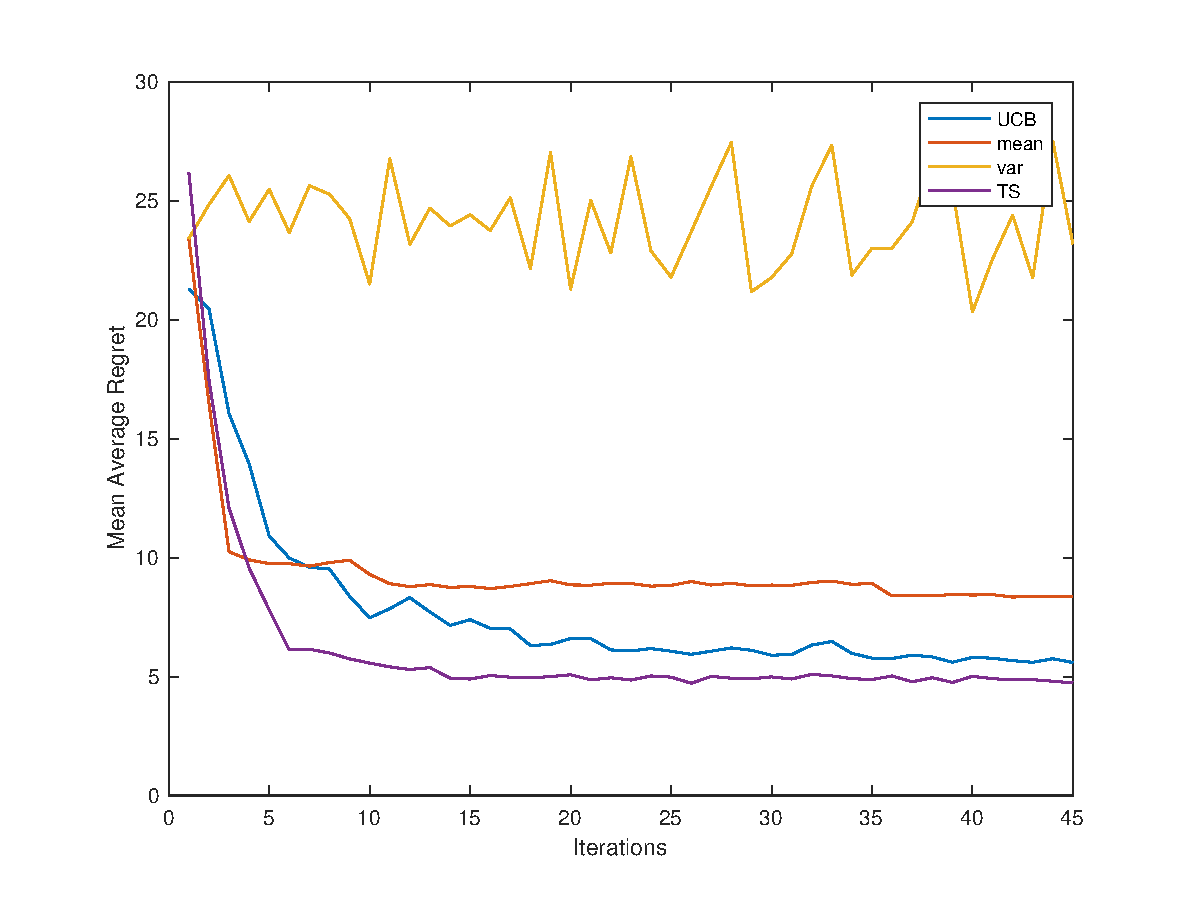
\includegraphics[width=1\linewidth]{figures/temperature_MC_150_kernel_empirical.eps} 
    \caption{Temperature data} 
    \label{temperature_data} 
    \vspace{4ex}
  \end{subfigure}
  \begin{subfigure}[b]{0.5\linewidth}
    \centering
    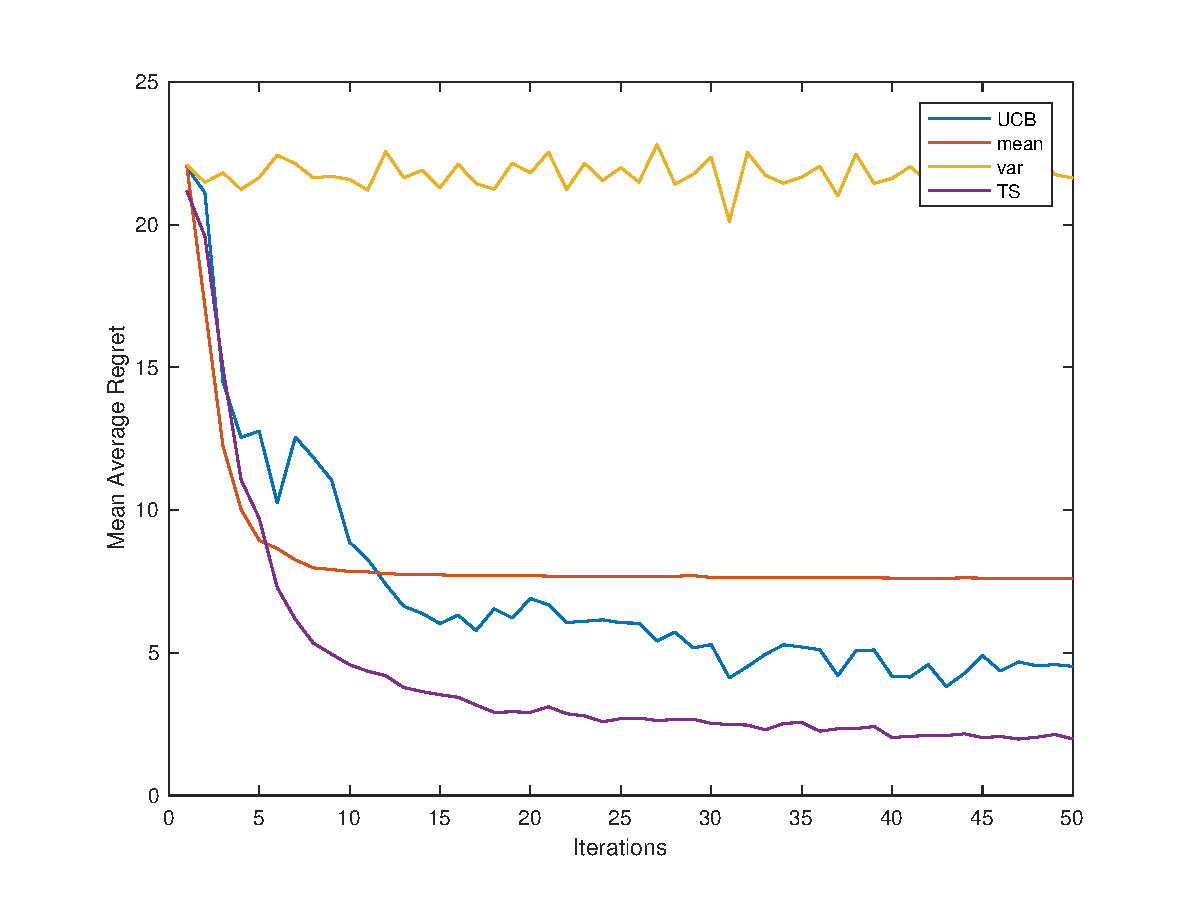
\includegraphics[width=1\linewidth]{figures/trafic_MC_360_kernel_empirical.eps} 
    \caption{Trafic data} 
    \label{trafic_data} 
    \vspace{4ex}
  \end{subfigure} 
 \caption{Comparison of performances: GP-UCB, TS-UCB and 2 naive heuristics on temperature data (a) and trafic data (b).} 
 \label{results_real} 
\end{figure}

\subsection{Analysis}

On Figures \ref{synthetic_data} and \ref{results_real}, one can see that GP-TS slightly outperforms GP-UCB on both synthetic data and real data. Naive heuristics which choose points with the highest variance or the highest mean have clearly and hopefully worse performances.


\section{Conclusion}

We have shown that a Thompson sampling algorithm for the MAB problem where the payoff function is sampled from a GP or has low RKHS norm, can have better performances than GP-UCB.

%\nocite{*}
\bibliographystyle{plainnat}
\bibliography{ref}

\end{document}